\documentclass[envcountsame]{llncs}
\usepackage[utf8]{inputenc}
\usepackage[american]{babel}
\usepackage[draft]{fixme}
\usepackage[square,numbers,sort]{natbib}
\usepackage{graphicx}
\usepackage{subfigure}
\usepackage{listings}
%\usepackage{color}
%\definecolor{natgreen1}{RGB}{50,93,61}
%\usepackage[colorlinks=true,urlcolor=natgreen1,linkcolor=natgreen1,citecolor=natgreen1]{hyperref}
%%%%%%%%%%%%%%%%% Functions for displaying code %%%%%%%%%%%%%%%
\newcommand{\billede}[3]{
  \begin{figure}[!ht]
    \begin{center}
      \IfFileExists{#2}{
        \includegraphics[angle=0,width=#1\textwidth]{#2}
      }{}
      \begin{minipage}{0.8\textwidth}
        \caption{#3}
      \end{minipage}
    \end{center}
  \end{figure}
}
\newcommand{\pcecode}[2]{
    \begin{figure}[!ht]
    \IfFileExists{#1.pce}{
        \lstinputlisting[%
        basicstyle=\tiny,%
        numbers=none,%
        numberstyle=\tiny,%
        language=Haskell,%
        tabsize=2,%
        commentstyle=\textit,%
        breaklines=true,%
        frame=single,%
        ]{#1.pce}
    }{}
    \caption{#2}
    \end{figure}
}
\newcommand{\code}[2]{
    \begin{figure}[!ht]
    \begin{center}
    \IfFileExists{#1}{
        \lstinputlisting[%
        basicstyle=\tiny,%
        numbers=none,%
        numberstyle=\tiny,%
        language=Haskell,%
        tabsize=2,%
        commentstyle=\textit,%
        breaklines=true,%
        frame=none,%
        ]{#1}
    }{#1}
    \begin{minipage}{0.8\textwidth}
    \caption{#2}
    \end{minipage}
    \end{center}
    \end{figure}
}
\newcommand{\repcode}[2]{
    \code{#1.rep}{#2}
}
\newcommand{\concode}[2]{
    \code{#1.con}{#2}
}
%%%%%%%%%%%%%%%%% Functions done %%%%%%%%%%%%%%%%

\title{Designing ERP 4 DJs}
%\subtitle{A Case Study}
\author{Femi Adisa\inst{1}, Jesper Andersen\inst{2}, Mikkel Thomsen\inst{2}, \and Morten Ib Nielsen\inst{2}\thanks{Supported by the Danish National
    Advanced Technology Foundation through the 3gERP project.}}
\institute{Center for Applied ICT, Copenhagen Business School\\Solbjerg Plads 3 DK-2000,
  Frederiksberg Denmark\and 
  Department of Computer Science, University of Copenhagen\\
  Universitetsparken 1 DK-2100, Copenhagen Denmark\\
  \email{fa.caict@cbs.dk, jespera@diku.dk, jonsson@diku.dk, mortenib@diku.dk}}

\begin{document}
\pagestyle{plain}
\maketitle
\begin{abstract}
TODO
\end{abstract}

\section{The Current Modus Operandi}
\label{sec:curr-modus-oper}

LejDJ.dk is a small online DJ and music equipment rental business,
whose services include the providing DJs for social events for
corporate and individual clients, and the rental of music equipments --
mixers, speakers, etc -- throughout Denmark. They cater for birthday
parties for all ages, anniversaries, weddings and company parties. 

The business of hiring and renting of DJs involves several processes
that make it interesting from a business process engineering
perspective. Despite its size, LejDJ’s activities include several
distinct business processes that present us with a unique opportunity
to be able to model these processes in the POETS architecture. Their
processes include: booking, equipment rentals, logistics, invoicing,
and billing.

LejDJ boasts a rich inventory of home-brewed software applications and
tools that enable them to record and monitor their day to day
transactions, from managing bookings to financials. There is an event
and DJ booking system, an invoicing system, spreadsheets for
accounting etc. However, these systems are silos of information and
even though the data contained within these systems are related and
crucial to the proper running of the business, they are not
inter-connected in anyway and data has to be manually extracted from
one system and painstakingly manually entered into another. While
these applications work very well on their own, errors -- omissions,
the wrong data in the right place, the right data in the wrong place --
when employees transfer data between these systems are inevitable and
in many cases only come to light when clients point them out.
Reconciliation is error-prone and with a company that handles over 500
events a year, an error of 1 percent will equal 5 jobs and this is
unacceptable.

In a bid to be closer to its customers and offer them localized
services, the company maintains 2 websites; one each for the Zealand
and Jutland regions. The underlying application is the same except
that each is customized to serve these two separate regions. Customers
do not choose which site to visit, but are instead redirected, based
on their IP address, to the site that serves their region. The
websites themselves both look have a uniform look and feel, except
that customers from Jutland are transparently handled by a Jutland
local, who is better familiar with the sub-cultural differences and
norms of the region, complete with accent. This forms part of the
company’s strategy of being close to the customers and offering
personalized services.

\subsection{The event booking scenario}

The process of booking a DJ for an event follows a series of events
that is initiated when a potential client contacts the company. This
initial contact can be either in the form of a phone call or via the
website. However, over 95 percent of contacts are done via the website
and the company encourages all clients to use the website. The
following steps are involved in the booking process initiated via the
website:

\begin{itemize}
\item A potential client fills and submits the contact us form via the
  website with their basic information and contact details such as
  name, address, phone number etc. and event information such as type,
  date, size, age group and demographics of guest. A canned response
  (auto reply) is sent to the customer, acknowledging the request and
  informing them to expect a response within 24 hours.
\item The information entered by the client is automatically sent to
  LejDJ’s gmail inbox, where it is automatically sorted through an
  extensive labeling system that determines if the client --
  identified by the email address -- is a new or a returning
  customer. In the case of a returning customer, a label will be
  attached that also indicates whether this correspondence by the
  returning customer is a new enquiry or a follow up to a previous
  enquiry.  The related correspondences are merged with the current
  one to form a message thread. This makes it easier to track the
  whole process from the initial enquiry until the event is finally
  booked or otherwise and also allows LejDJ to recognize who the
  particular client is. It is important to note that the feature that
  matches the email address of returning customers to their previous
  correspondence is an intrinsic gmail feature that uses google apps
  that was configured by the company; however this feature is not
  available in their own database system. Gmail also generates a file
  with all the info entered by the customer and this is then entered
  by hand into LejDJ’s booking system, in the case that the client
  books the event.
\item Following a series of correspondence, during which the client
  and LejDJ negotiate and renegotiate the terms of the engagement and
  an updated invoice is sent to the customer for approval.  Should the
  client choose to book the event with LejDJ, it is then entered into
  the Booking system and labeled in the gmail system as booked. This
  also triggers a series of processes and tasks, including booking the
  actual DJ that will play at the event and the logistic for
  delivering the right equipments to the event venue, at the right
  time.
\item The booking process is completed by the generation of an order
  confirmation/invoice that is sent by email to the customer. This
  contains the amount to be paid and payment due date, which is
  usually within 8 days after the event for private clients and 45
  days for corporate clients.
\end{itemize}


\paragraph{Events Booking system Pain Points}

The current booking system comprises 3 to 4 different vanilla
applications that share the same data but do not share one integrated
database. Currently, data is pulled from one system and entered into
the other manually. There is the gmail application that receives the
enquiry emails and keeps details of all email correspondence in its
own customer file. There is the application developed in Access that
all data about booking is transferred as soon as the customer decides
to book the system. A rental/DJ booking system is where the DJ and
equipment is booked for the particular event. Finally, an invoice is
generated by collecting information from the event booking and
Rental/DJ booking systems and combining them into a PDF file, which is
then sent as an email attachment from Microsoft Outlook. Below are the
pain points identified with the booking process:

\begin{itemize}
\item The manual entry of data between the gmail application and the
  local booking system is done through a copy/paste operation.  An
  automated/integrated operation is desirable.
\item Correspondence from returning customers is automatically
  recognized in the gmail application through the email address, and
  is matched accordingly with any previous correspondence; this is not
  done in the Access system.
\item The identification of returning customers on several levels, and
  not from email address alone is desirable. Returning customers who
  write in using another email address for example are not recognized.
\item Fragmented/incomplete/inconsistent/redundant customer
  information as a result of copying and pasting from one system to
  another.
\item The automation of the order confirmation and invoicing
  process. The system should be able to pull the necessary data for
  generating the invoice and send this automatically to the client.
\end{itemize}

\subsection{DJ booking Scenario}

The process of booking a DJ for a confirmed event is handled by one
and only one employee, and is based on tacit knowledge and or
favoritism. LejDJ has a group of DJs that are affiliated to it. They
subscribe to the company in order to get gigs; DJs are supposedly
picked for events based on the event type and the intended audience,
which will influence the kind of music to be played and hence the DJ.

DJs can choose to bring their own equipment or rely on LejDJ to
provide and deliver the sound equipments on-site and on-time. Some DJs
have in their possession, equipments belonging to LejDJ which they
bring along to events. Either way, DJs that use LejDJ equipments are
the preferred choice when it comes to choosing a DJ for an event. DJs
that chose to bring their own equipment are way down in the pecking
order when it comes to selecting DJs for events. This is in line with
the company’s means at minimizing costs. The payment structure is as
follows:

\begin{itemize}
\item 2000Dkk for of a 5-hour show for DJs who use some of LejDJ’s
  equipments that is delivered to the event site either by themselves
  or by LejDJ.
\item DJs that have and bring their own equipments to events are paid
  2500Dkk for the same 5-hour show. However, they are less preferred.
\item DJs who use all of LejDJ equipments earn 1500Dkk depending on
  their experience.
\end{itemize}

Shows that run over the agreed time are normally priced at 300Dkk per
hour. LejDJ tries to follow a 5-hour booking slot for events but
customers can ask for anything from between 4 hours to more than 5
hours, in which case it will be priced at the hourly rates. Customers
wanting to book an event for 3 hours or less are charged a premium
flat rate -- usually negotiable.

DJs are usually paid by LejDJ after the event is completed, with the
amount transferred directly into the DJ’s account. Sometimes, the
client will give cash to the DJ at the end of an event and the DJ
would simple subtract their dues and remit the difference into LejDJ’s
account or hand over cash to an employee.  There are rare events where
a DJ would decline payment for a job on the basis of their feeling of
not having done a satisfactory job -- in other words, they did not feel
they got the crowd jumping. 

Once the DJ has been chosen for an event, the employee first places a
call to the DJ to ascertain his availability. If the chosen DJ is not
able to play at the event, another DJ is chosen and the process is
repeated. Thereafter, the customer and event information – type,
place, time, expected number of guests, demographics - is pulled from
the event booking system. This information is combined with the DJ
information and used to generate an event sheet that is sent to the DJ
and also the employee in charge of booking the equipments, in the case
that equipments are required.

The DJ booking system is the same one that is used for booking
equipments for events.

\paragraph{DJ Booking system Pain Points}

\begin{itemize}
\item Automating the DJ selection process.
\item A rating system for DJs that can be taken into consideration in
  the selection process.
\item A standardized method of payment. Ideally, one that eliminates
  the use of cash is highly desirable.
\item LejDJ would like customers to pay directly into their account
  instead of handing over cash to DJs at events, but they also realize
  that discouraging clients from paying to the DJs at the end of
  events could lead to a longer waiting period for payment.
\end{itemize}

\subsection{Payments}

The whole payment process for events handled by LejDJ is very
fragmented and sometimes makes it difficult to correctly track and
record payments and reconcile accounts.   Customers rarely pay upfront
for events and LejDJ gives a grace period of 8 days for private
customers and 45 days for corporate customers, to pay for an event.
However, several usually scenarios arise; Private customers often pay
late and in chunks, and this poses a multi-faceted problem for LejDJ
and corporate customers can forget to pay.

The invoice sent out to private customers after the confirmation of an
event states that payment for an event has to be made within 8days.
However, several payment scenarios can occur:

\begin{itemize}
\item Some customers will pay the DJ at the end of the event in cash;
  in such a case, the DJ subtracts his fee and remits the rest back to
  LejDJ’s account or hands over cash to an employee.
\item Most customers will pay within the 8-day period.
\item Some customers fail to pay within the 8-day period. In this
  case, LejDJ gives a 14-day - from event date - grace period and then
  sends a reminder stating another 8-day period. If payment is not
  effected, the customer is sent another reminder 14 days from the
  date of the first reminder, giving another 8-day period to effect
  payment. This 8-14 days cycle is repeated three times.  Should the
  customer fail to pay after the third reminder is sent out, a formal
  letter is sent out to the client, stating that LejDJ will seek legal
  redress.
\end{itemize}

In the case of corporate clients and usually due to lots of companies
having a payment policy that requires a 45-day waiting period, LejDJ
gives a 45-day period for corporate clients to pay for an event.
However, if the company fails to pay and LejDJ has to send another
reminder, they still have to wait another 45 days to find out if they
have been paid or not. This represents a very long period for such a
small company.

DJs are usually paid the next working day after an event, regardless
of whether the customer has paid or not. As mentioned earlier, DJs
that receive payment from clients after an event will usually subtract
their fee from the payment and remit the reminder to LejDJ’s account
or hand over cash to an employee.

All payment transactions are recorded and handled in Microsoft excel
sheets. This requires a lot of copying and pasting of customer and
event data. Information can be spread across multiple sheets and it is
difficult to integrate data and errors can often occur. Reconciliation
of fragmented payment is also a problem.

\paragraph{Pain points for payments system}

\begin{itemize}
\item During the course of negotiations, LejDJ can sometimes give a
  discount to the client. The employee can sometimes forget to record
  such in the system and this creates discrepancies in records and
  often times lead to embarrassing situations when LejDJ demands the
  missing sum from the customer.
\item Most of the payment records right now is handled in an excel
  sheet. It is difficult to update multiple instances of a single
  payment, where such records occur in several sheets.
\item The way DJs are paid is very unstructured and inconsistent.
\item It is difficult to get an overview of financial transactions –
  payments and expenditures.
\item The current excel based system offers no budgeting and
  forecasting facilities.
\item It is not very easy to track which customers have paid their
  outstanding, especially with the fragmented and inconsistent ways of
  payment.
\item Reconciliation of partial payments across several sheets.
\item Integration of financial information across multiple sheets.
\item Because expenses are currently recorded in excel sheets, the
  company has no way of knowing exactly where they stand in terms of
  expenditure against earnings at any particular point in time.
\end{itemize}

%%%%%%

% The DJ booking
% \begin{itemize}
% \item Late payment from customers
% \item Very limited tracking of financial transactions
% \item No tracking of monthly expenses or revenue
% \item Payment of/from DJs is unstructured/inconsistent
% \item No budgets or forecast
% \item Fragmented/incomplete information about customers, such as
%   event-address and invoice-address.
% \end{itemize}

% The rental of equipment
% \begin{itemize}
% \item No inventory tracking
% \item Very limited tracking of financial transactions
% \item Little customer info
% \item No fixed-line internet connection in warehouse (this is really
%   more a constraint than a pain point)
% \end{itemize}


% \subsection{Financial statistics}
% The system will support a number of financial reports for the company
% to use. These include:
% \begin{itemize}
% \item List of events sorted by event type
% \item List of outstanding event
% \item List of outstanding invoices
% \item Revenue and amount of event sorted by the DJ
% \item Revenue and amount of event sorted by location. I.e. event in a
%   specific city.
% \item List of quotes not yet converted into binding contracts
% \item Budgeting information
% \end{itemize}
% These reports will be available when the user presses the button
% ``reports'' on the button of the screen in
% Figure~\ref{fig:mainscreen}.

% The system also supports dynamically aggregated information for
% individual entities such as DJs or customers. This information is
% available on the entity information screen

\section{Customizing POETS for the DJ case}
\label{sec:build-poets}
\subsection{Case story}
\label{sec:case-story}
Based on correspondence with the customer, a sales quote is created in
the system by clicking on ``enter new contract'' and selecting type
``quote''. If the customer decides to accept the quote it is converted
into a legally binding contract. The contract contains:
\begin{itemize}
\item Customer information including name, address, phone number,
\item Event information including date, location, type (wedding,
  birthday, etc.), gear requirement, DJ and size.
\item Accounting information including price, DJ payment, payment
  grace period.
\end{itemize}
The decision of which DJ will play the event is not modelled in the contract, and is an decision made by the company based on event type and availability of DJs.

The contract is now in the system and can be viewed by querying for
open contracts. As there are no outstanding deliverable, only the
payment remains of the contract. This is either handled by the DJ at
the event or by the customer wiring the payment to the Company within
the payment grace period. If the DJ is paid on the spot, he can go
into the system and flag the event as paid. The DJ and the Company
will then enter a contract where the DJ is committed to deliver the
payment for the event to the Company.

If the payment is not received on time the Company will start to issue
reminders with a 14 day cyklus. The customer has 8 days to pay, and 6 days grace period before another reminder is issued. After three reminders are sendt, a formal letter is sent to the customer with descriptions of what legal measures the company will resort to if the invoice is not paid.

%% Copied from my thesis draft -- Mikkel
In this case study, the business process will be divided into three
parts: The sales process, the DJ booking process, and the payment
process. The sales process starts with the customer initiating
contacts to the company and finishes when the event is booked. The booking of DJs is the process of choosing the right DJ for the job and making sure that he or she is available. The payment process starts when the DJ finishes the job and includes the possibility to pay the DJ in cash on the night of
the event. To model this, an extra loop will have to be created during
the payment sub-process. The three models can be seen in
Figure~\ref{fig:FourDJsSales}, Figure~\ref{fig:FourDJsDJ}, and
Figure~\ref{fig:FourDJsPayment} respectively.

\billede{0.55}{FourDJsSales.pdf}{Process diagram for the 4 DJs sales
  process \label{fig:FourDJsSales}}
\billede{0.55}{FourDJsDJ.pdf}{Process diagram for the 4 DJs DJ
  selection process \label{fig:FourDJsDJ}}
\billede{0.55}{FourDJsPayment.pdf}{Process diagram for the 4 DJs
  payment process \label{fig:FourDJsPayment}}

In Figure~\ref{fig:FourDJsPayment} a choice is being made whether the
DJ receives the payment or the customer pays via invoice. I the former
case, by receiving payment the DJ enters a contract with the company
to transfer the payment for the event to the company, deducting his
own salary.

To model the above processes in the POETS sýstem, we use two contract templates. This is due to the fact that the decision of which DJ to assign for an event is not taken when the contract is entered with the customer. Therefore we define a contract template stating that the customer must find a DJ and assign him or her to the event. When a DJ has been found, a \textit{three party contract} is entered with the company, the customer, and the DJ obligating the DJ to play the event, the company to pay the DJ, and the customer to pay the company. All at specified deadlines. To ease the transferring of data between the two contracts, we construct an ontological entity called \textit{EventInformation} containing all information about the event, including data, time, type, size, etc. In addition to the EventInformation entity, the contracts contains the appropriate agents.

Figure~\ref{pce:FourDJsSales} is an example of the contract ontologies for the two described contract templates (called \textit{EventContract} and \textit{DJContract} respectively). The POETS contract templates implementing the processes
can be seen in Figure~\ref{code:FourDJsSales}.

\pcecode{FourDJs}{Data model for the 4 DJs sales and payment
  processes.\label{pce:FourDJsSales}}

\concode{4djs}{POETS contract implementing the 4 DJs sales and payment
  processes.\label{code:FourDJsSales}}

% \subsection{Financial reporting}
% Financial reporting is marked as a pain point in the 4 DJ case study
% with focus on short term statistics, especially an overview of the
% monthly income and expenses. Beside the mandatory financial reports a
% new report must be defined as the aggregation of the currency of all
% \emph{Payment} events that has occured within the last month. An
% example of a report in the POETS reporting language can be seen in
% Figure~\ref{rep:monthly}.

% \repcode{FourDJsMonthly}{POETS report for displaying monthly
%   income.\label{rep:monthly}}

% In their present system, expenses are tracked manually in a
% spreadsheet by the financial manager. These expenses include DJ
% salary, transport expenses (gas, insurance etc.), food, repairs,
% purchasing of new gear, and advertisement.  The DJ salary is handled
% by the payment section in the DJ contract in
% Figure~\ref{code:FourDJsSales}. The rest of the expenses are handled
% by standard purchasing contracts. An example of a report displaying
% monthly expenses cen be seen in Figure~\ref{rep:monthly}.

\section{Conceptual GUI design}
\label{sec:gui-design}
Before a user can log on to the system a user profile must be created
by a super user (see Figure~\ref{fig:createuser}).  A user profile
specifies a set of permissions as well as the layout of the GUI. The
system has several default profiles, called \emph{roles}, which
simplify the process of defining permissions and default
layouts. While permissions must be granted by a super user, users
themselves can change the layout of their GUI.

With a user profile in hand the user can log on to the system (see
Figure~\ref{fig:logon}). Upon successful login the user is presented
with the \emph{main screen} (see Figure~\ref{fig:mainscreen}).

\subsection{The Query Field and Saved Searches}
\label{sec:query-field}
The main screen has two parts. On top is the \emph{query field} and
\emph{query button} and below the \emph{shortcut space}, which is
empty in its most basic form\footnote{Not entirely true, cf. \emph{The
    Static Shortcut Space}.}.

The query field, inspired by Google, accepts searches written in a
simple domain specific query language, which we describe in
Section~\ref{sec:doma-spec-query}. Whenever a search is performed, the
user can choose to save the search, if it has not already been saved,
by assigning an icon, a name, and possibly several tags\footnote{Tags
  can be used to group related saved searches and have icons and
  names, but not tags themselves.} to it. This is done via an overlay
(see Figure~\ref{fig:savesearchoverlay}), that appears once the
\emph{Save Search} button is clicked. Together saved searches and tags
are called \emph{shortcuts}. Once saved they become available on the
shortcut space.

The shortcut space, inspired by iPhone / Android, has two parts: 1. a
page space with room for $4\times 4$ shortcuts per page (navigation
between pages is done using gestures), and 2. a static space with room
for $1\times 4$ shortcuts - two of which are the predefined
\emph{Enter contract} and \emph{View report} shortcuts described in
Sections \ref{sec:enter-new-contract} and \ref{sec:reports}
respectively.

\begin{figure}[bth]
  \subfigure[Creating new users.]{\label{fig:createuser}
    {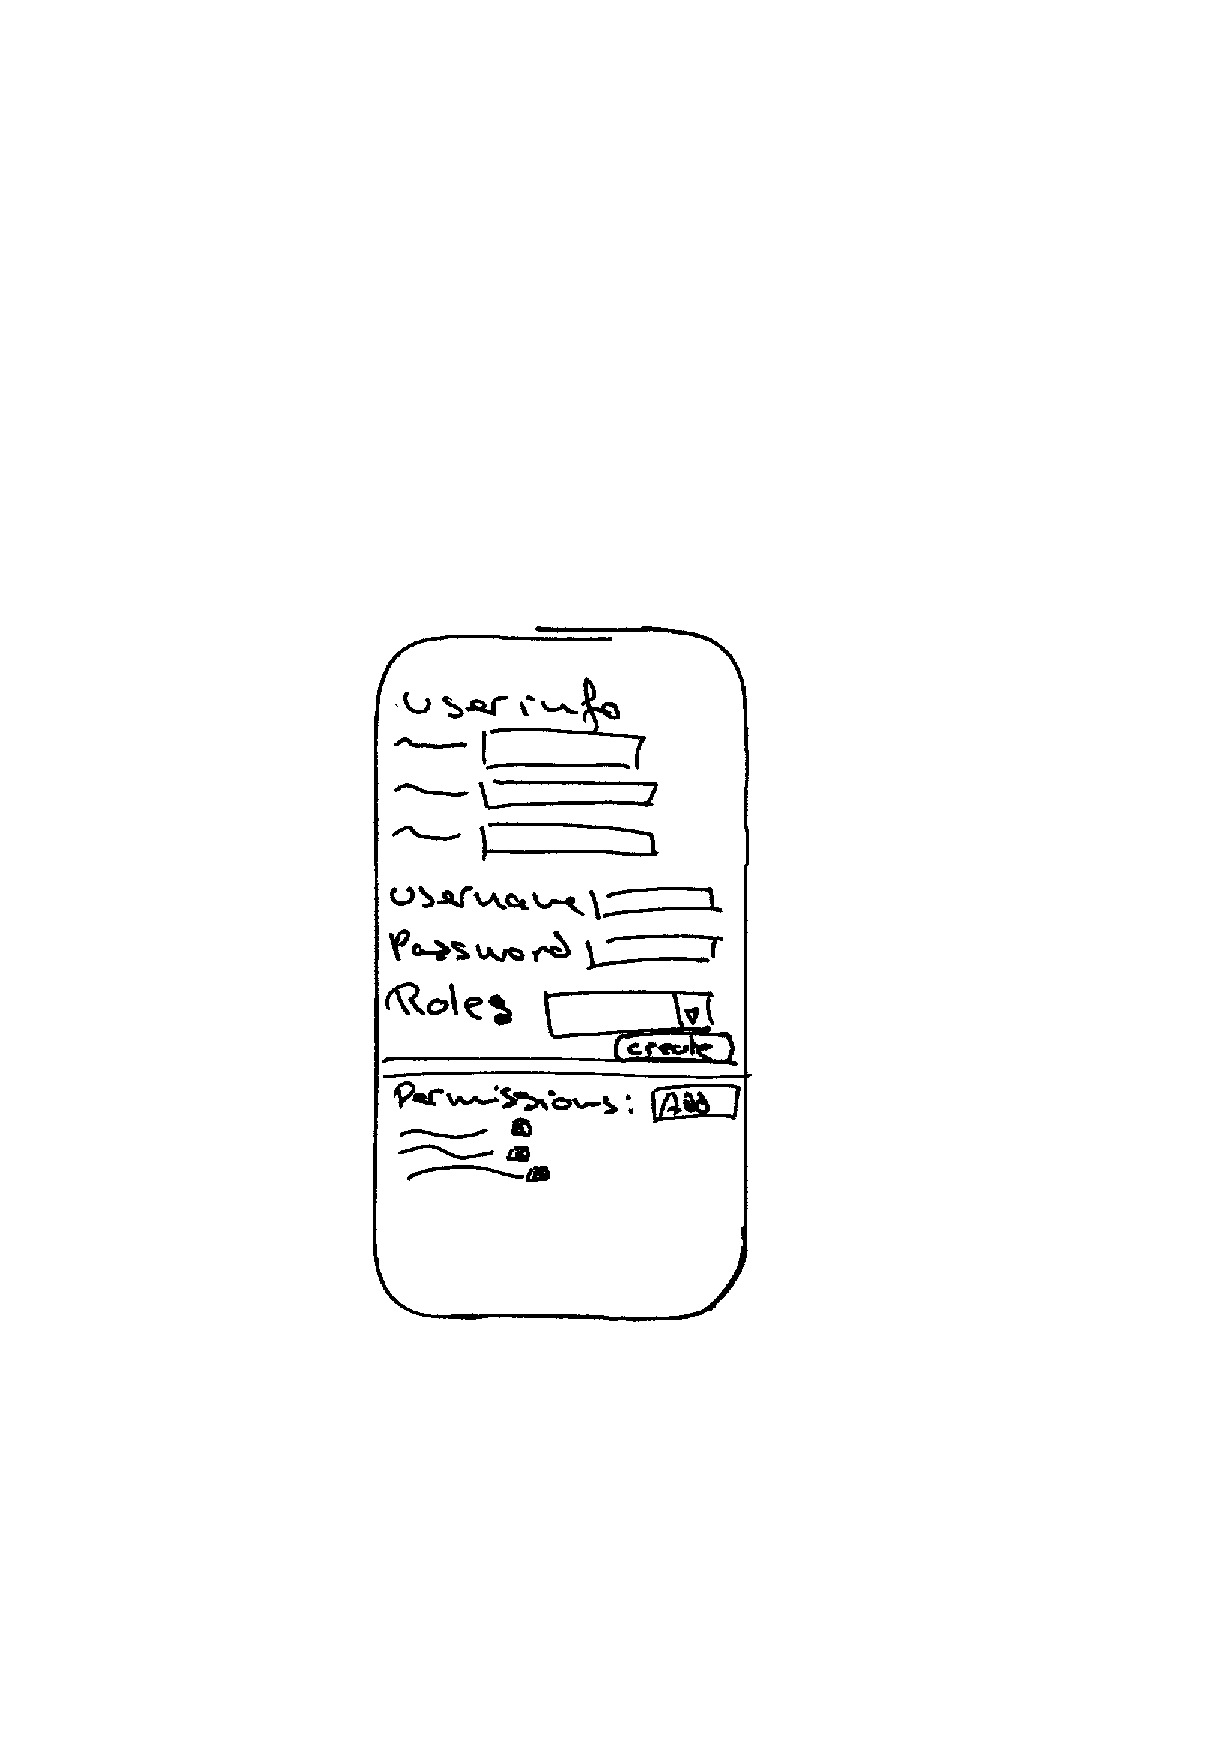
\includegraphics[scale=0.80]{gfx/createuser}}} \quad
  \subfigure[The logon screen.]{\label{fig:logon}
    {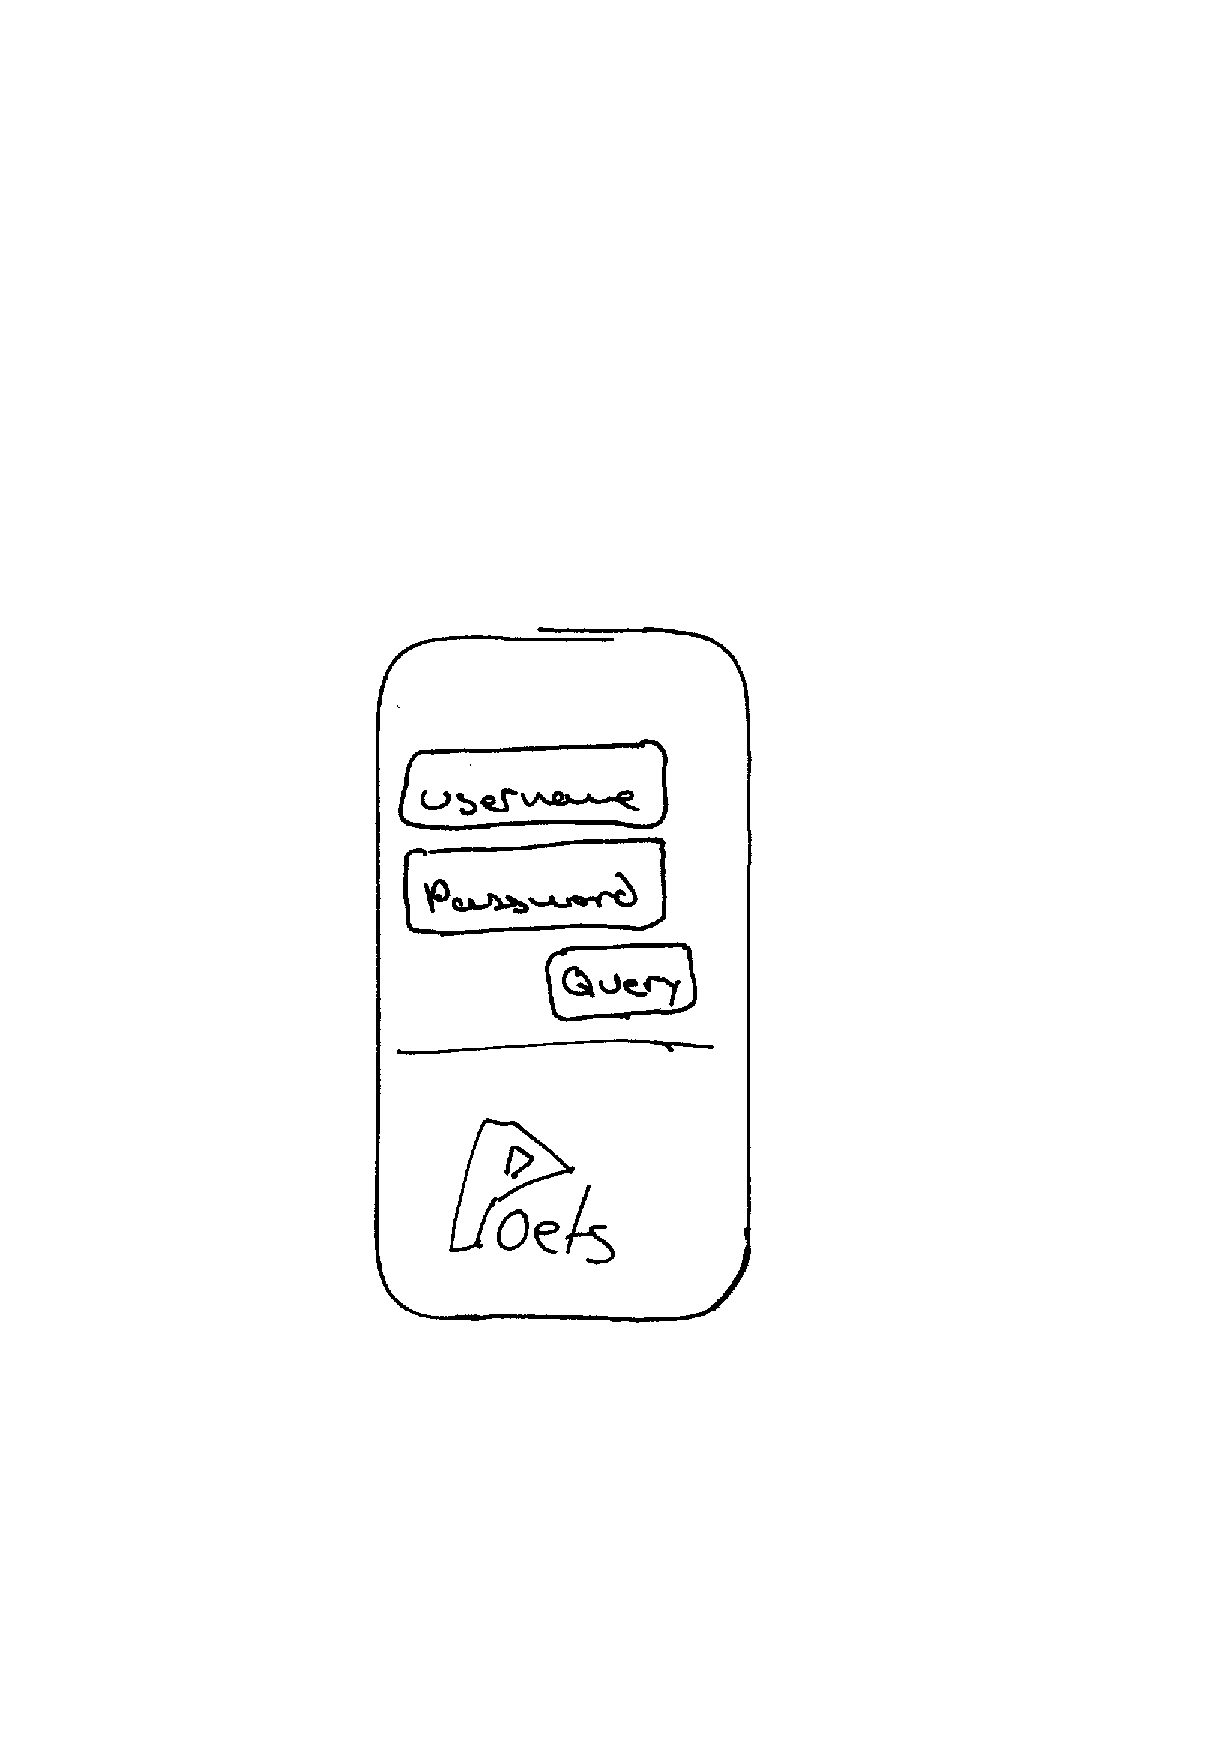
\includegraphics[scale=0.80]{gfx/logon}}}\\
  \subfigure[The main screen.]{\label{fig:mainscreen}
    {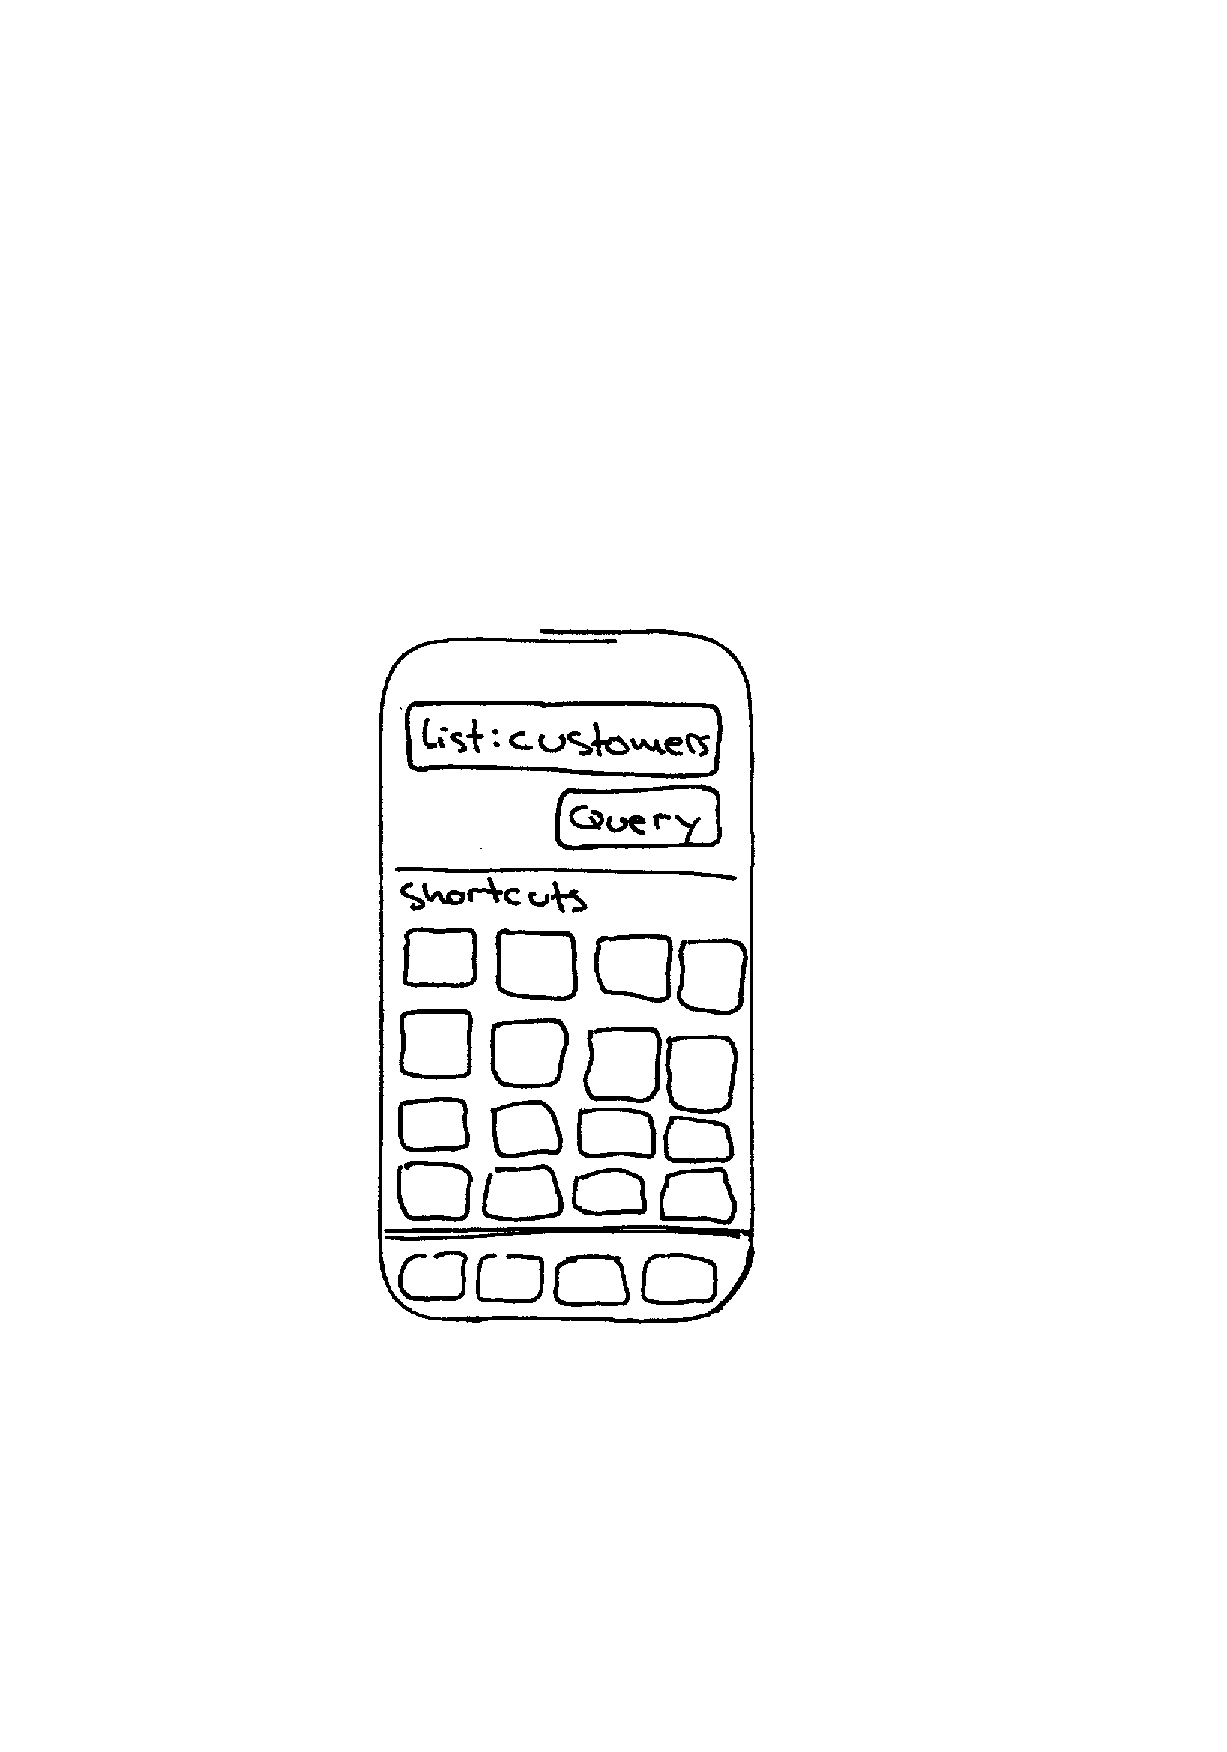
\includegraphics[scale=0.80]{gfx/mainscreen}}} \quad
  \subfigure[Search results.]{\label{fig:searchresult}
    {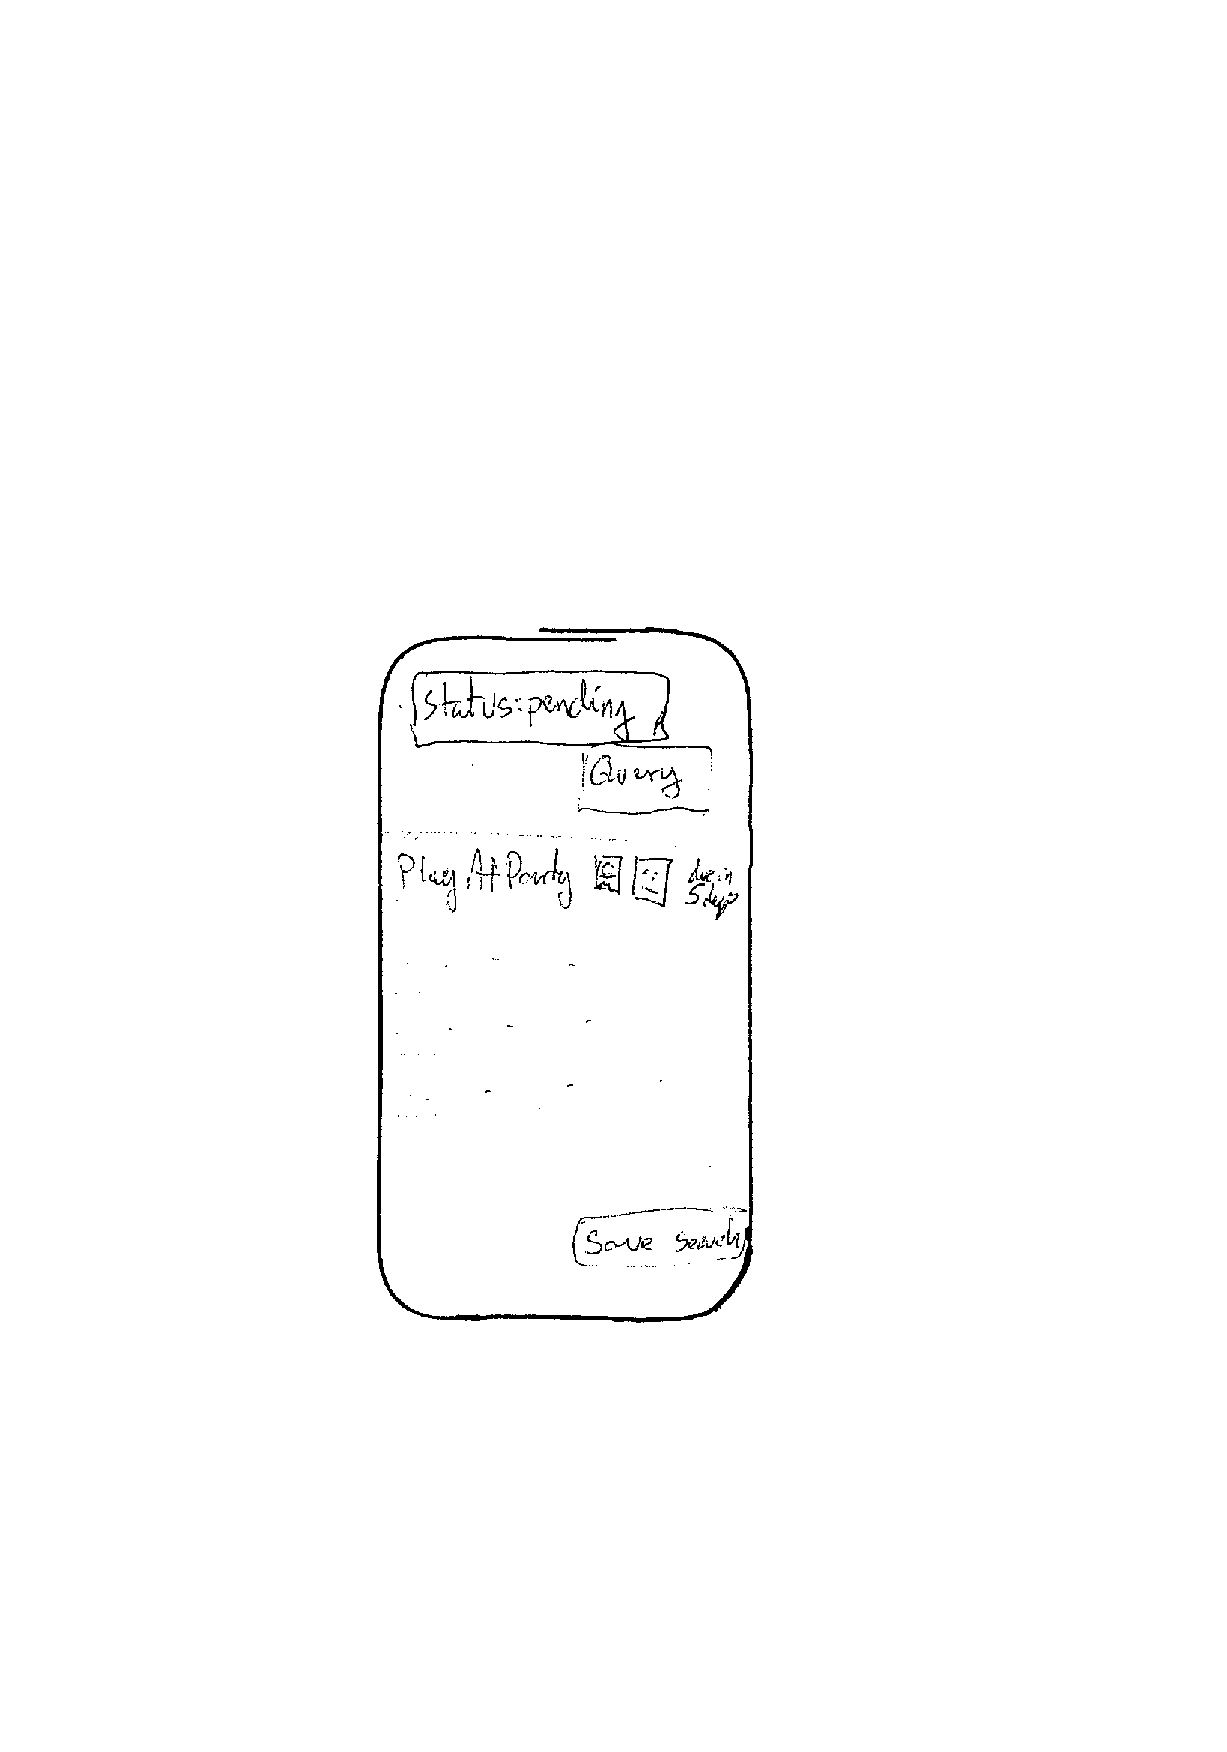
\includegraphics[scale=0.80]{gfx/searchresult}}}
      \label{fig:first4}\caption{}
\end{figure}

\begin{figure}[bth]
  \subfigure[The contract view.]{\label{fig:contractview}
    {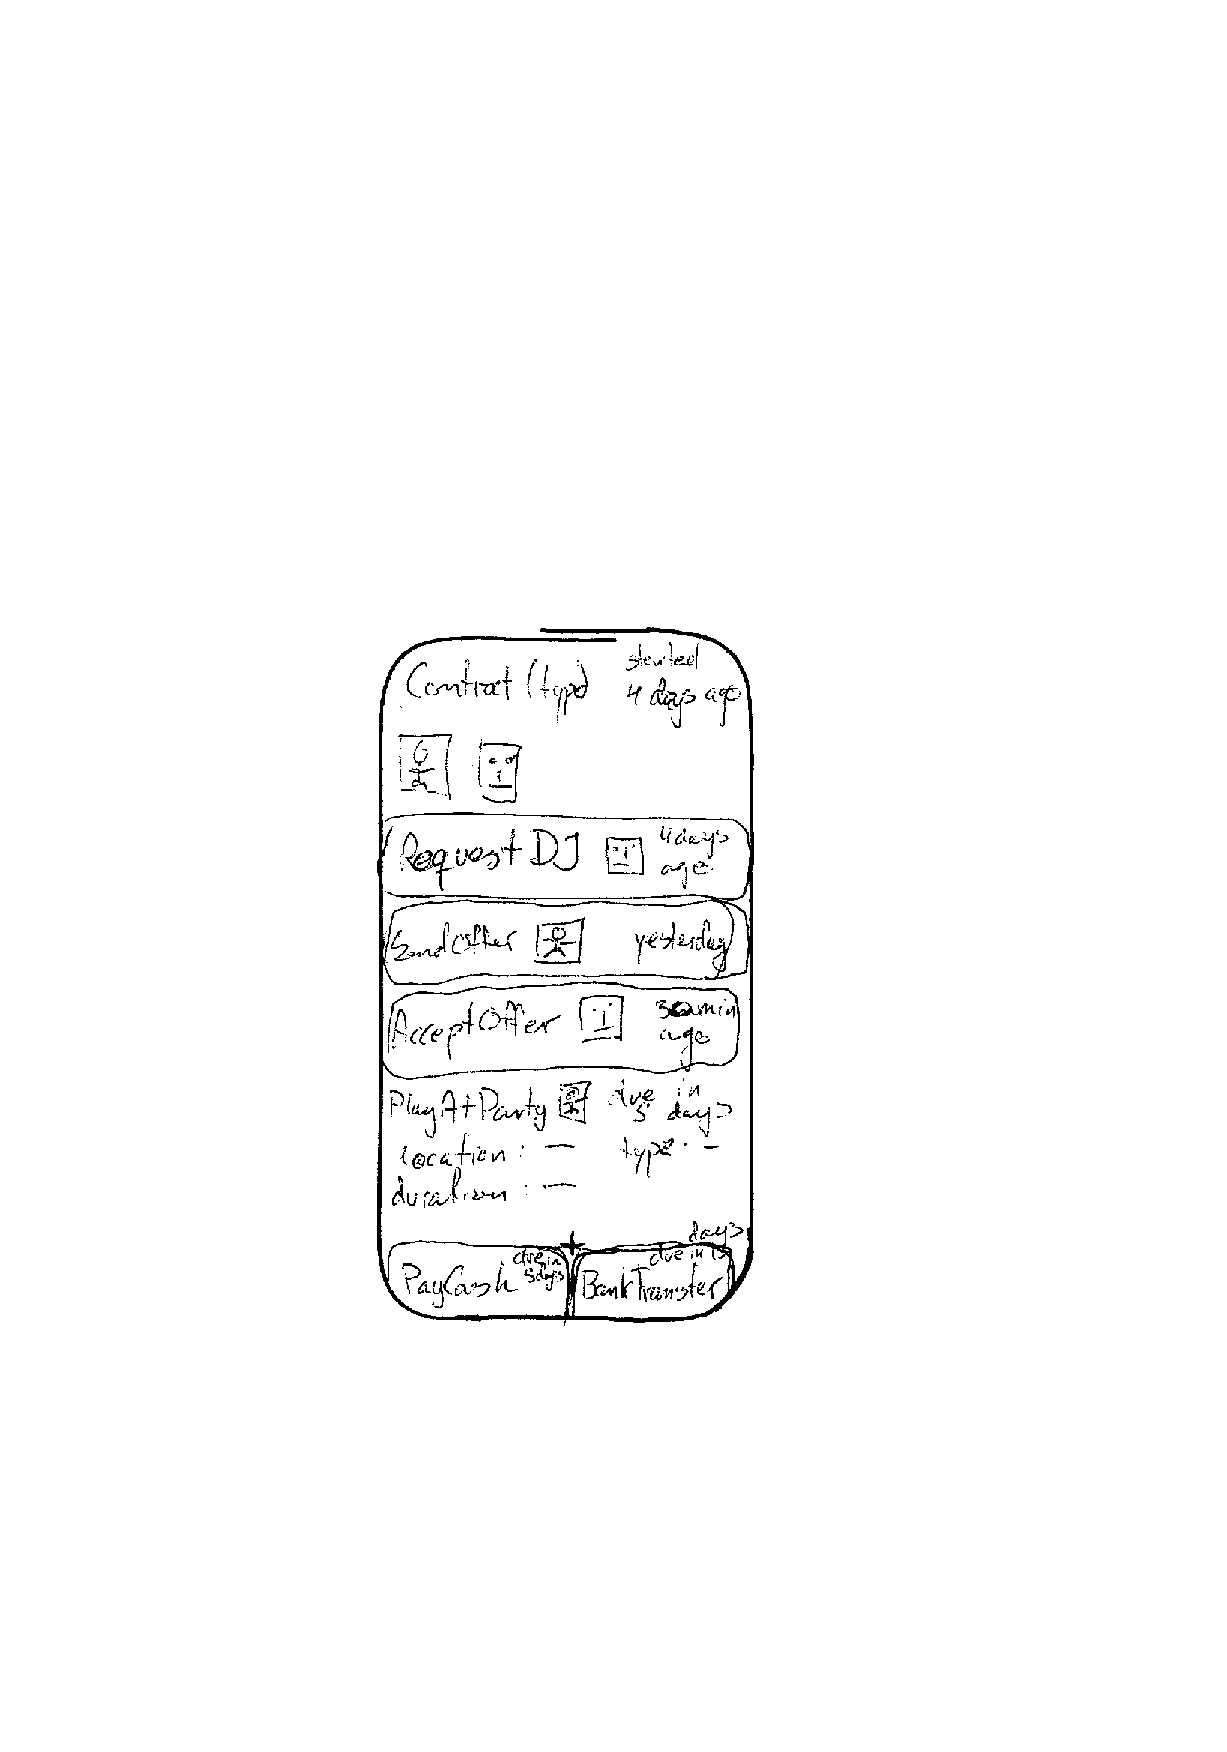
\includegraphics[scale=0.80]{gfx/contractview}}} \quad
  \subfigure[Overlay for saving
  searches.]{\label{fig:savesearchoverlay}
    {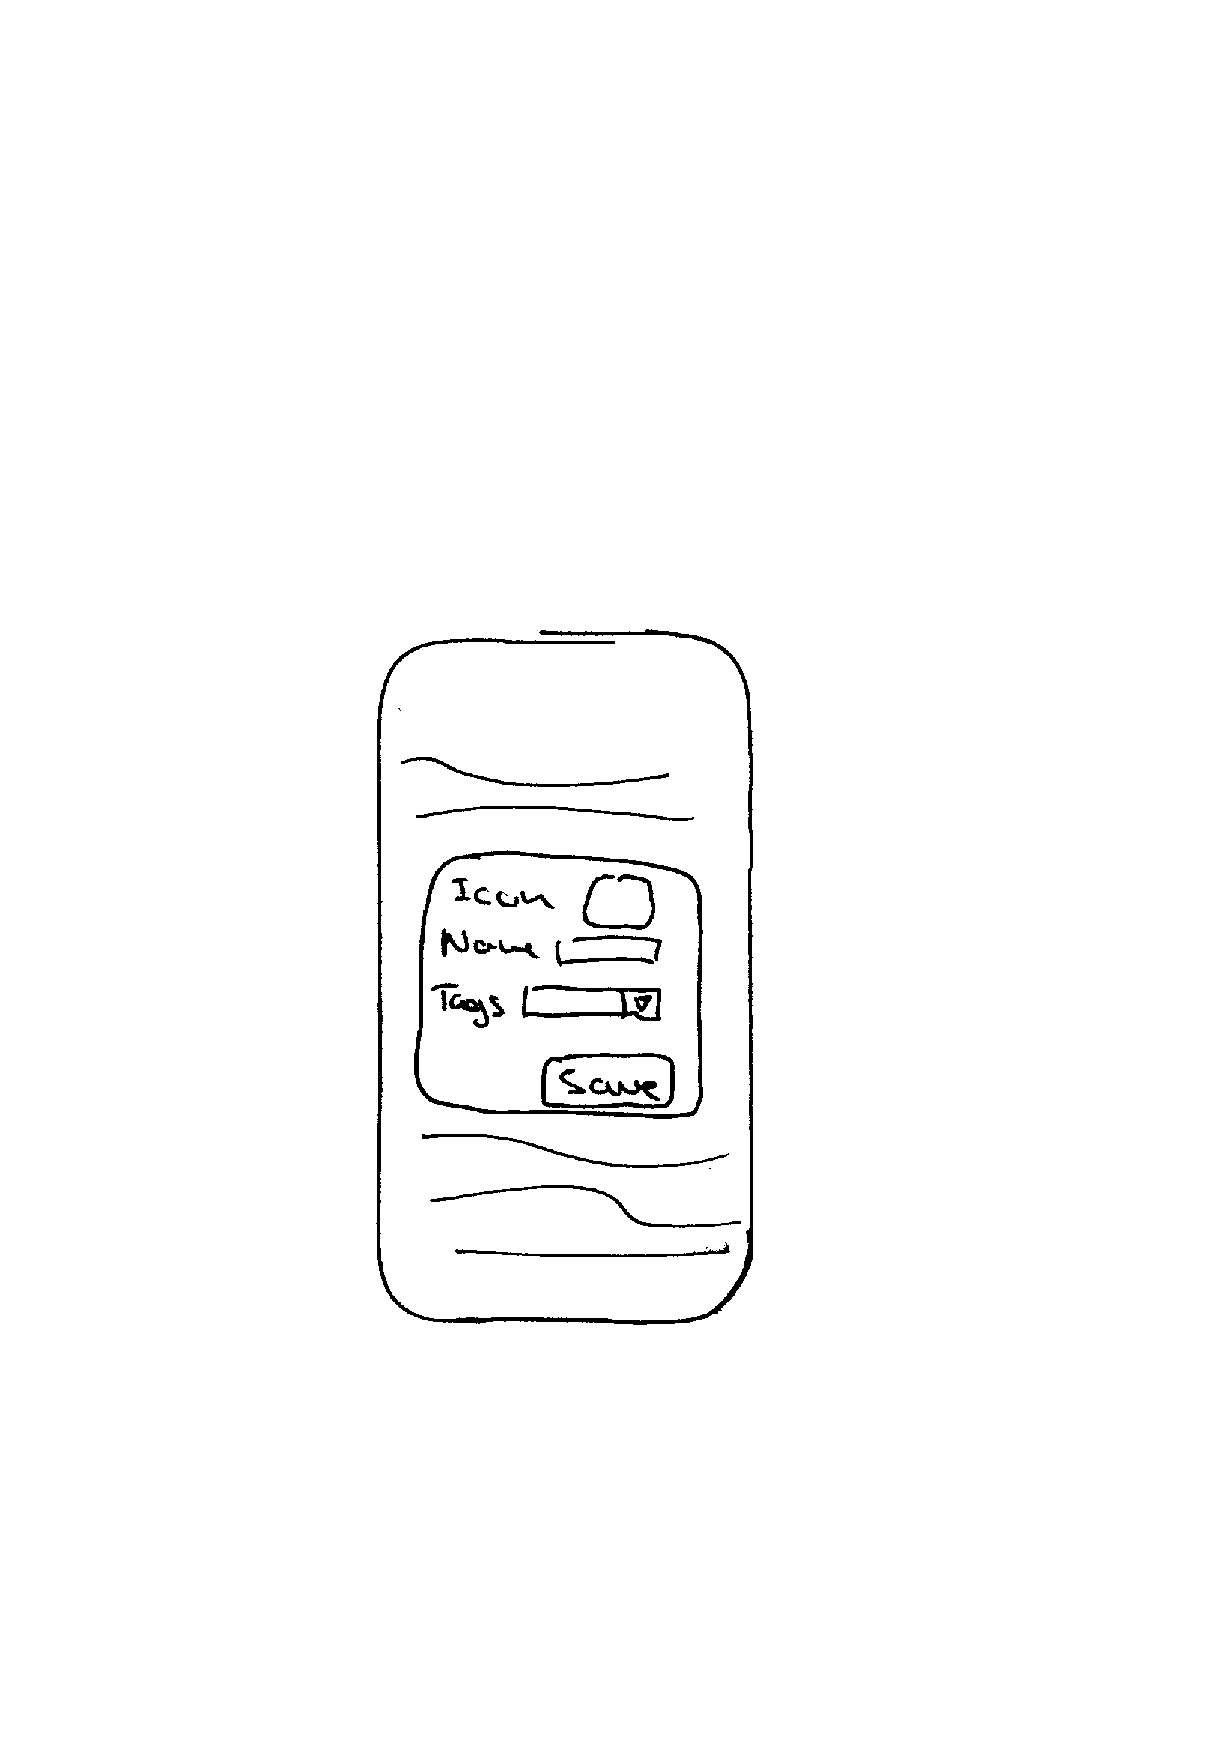
\includegraphics[scale=0.80]{gfx/savesearchoverlay}}}
      \label{fig:first5}\caption{}
\end{figure}

\subsection{Interacting with search results}
\label{sec:interact-search-results}
The result of the search query is shown below the query field and
button replacing whatever was previously displayed in that
space. Suppose the search query is \texttt{status: pending}. The
result of pressing the 'Query' button is a set of tasks that should
(could) eventually be performed according to the contracts that have
already been entered into.

The resulting set of tasks is displayed in a list. Each list-entry
displays a summary of the task containing information about the kind
of task (a delivery, a payment, DJ'ing at a party, etc.), who is
responsible for performing the task, and the latest due date of
performing the task. An example of how this could look is seen in
Figure~\ref{fig:searchresult}.

At the bottom of the list-view is a button for saving the search query
as a shortcut. Pressing the ``save search'' buttons opens a page where
the user can fill in information about the shortcut as mentioned in
Section~\ref{sec:gui-design} and illustrated in
Figure~\ref{fig:savesearchoverlay}.

Clicking a list-entry opens a page with information relevant to the
list-entry. In this case, the list-entries represents tasks to
perform, so the page opened is a view on the contract prescribing that
the particular task should (could) be performed
(Figure~\ref{fig:contractview}).

\subsection{The contract-view page}
\label{sec:contractview}

The contract-view page displays information about the legal entities
that have entered into the contract as well as information about the
previous events related to the contract and future tasks that must be
(can be) performed according to the contract. The contract-view
additionally allows the user to mark (only) the tasks that are
stipulated in the contract as performed.

In Figure~\ref{fig:contractview} the contract-view page is split in 3
main parts: 1) static information about the contract (legal entities
and the start date of the contract), 2) a log of previous events, and
3) the future tasks that must (can) be performed.

The future tasks is again split in two parts: 1) the tasks that can be
performed now and tasks that should eventually be performed but which
depend on other tasks (or events occurring) being performed first.

Tasks and events are visualized in a task-event-view which displays
information about the task or event. The information displayed is
mostly dependent on the kind of task/event. A 'Payment' task will show
information about the amount to be payed. However, all tasks have an
associated deadline and legal entity. The deadline states the latest
time at which the task must be performed and the legal entity
describes who is responsible for performing the task. When a task is
marked as performed it is logged as an event. One can view a performed
task as an event. An event contains the same information as the
corresponding task, except the deadline is instead a timestamp
indicating when the task was performed. 

A task-event-view can be either open or collapsed. The collapsed
variant shows only summary information about the task/event: kind,
responsible, and deadline/timestamp. By default all logged events are
shown collapsed. All tasks that can be performed now are shown in the
open state displaying all the information associated with the
task. All future dependent tasks are shown collapsed. Clicking a
collapsed task-event-view puts it into opened mode. Clicking the
'header' part of an open task/event puts it in collapsed mode.

If more than one task can be performed now all of the potential tasks
are laid out horizontally next to each other. Otherwise tasks (and
events) are stacked on top of each other vertically.

\subsection{Entering a new contract}
\label{sec:enter-new-contract}

From the static shortcut space visible on the main screen the user can
press the \emph{Enter contract} button. Pressing this button opens a
mostly empty contract-view page. On the page the user can select the
contract type (from a set of predefined templates). Any contract must
contain information about the legal entities which have agreed to
enter into the contract. By default the legal entity represented by
the user of the system is added to the list of legal entities of the
contract. Additionally all contracts have a start date. Depending on
the contract template more information may be needed. A sales contract
could need information about the goods being exchanged and the agreed
price. Once all static contract information has been entered, the
contract-view page is updated to show the currently pending and future
dependent tasks as outlined in Section~\ref{sec:contractview}.

\subsection{Reports}
\label{sec:reports}
In ERP, the term \emph{report}\fixme{A report is composed of
  \emph{content} (report data) and \emph{layout} (visualization of the
  content)} refers to the \emph{data} that goes into a business report
as well as the \emph{visualization} of that data (i.e., two different
visualizations of the same data constitute two reports).  In POETS we
make a clear distinction between the two. It is the task of the
\emph{reporting engine} to compute the data, whereas the visualization
of data is delegated to another subsystem\footnote{Currently offered
  as a student project.}.

One major way in which POETS differs from contemporary ERP systems
such as SAP and NAV is that POETS does not use a relational database
design to support business objects (e.g., customer and product lists,
balance sheets, etc.). Instead business objects (i.e., data) are
computed on demand using reports\footnote{This is feasible with
  respect to running time because of the way the reporting engine
  works (incrementalization).} and then visualized as appropriate
(e.g., as lists with which one can interact or as PDFs for print).

As an example the query \texttt{list: customers} triggers a report
that computes a data object containing the list of customers. Once
computed this data object is visualized (as a list) in the
GUI. Similarly \texttt{status: pending} triggers a report that
computes a data object containing the list of all pending event.


\subsubsection{The final list of all reports needed}
%%%% The final list of reports

This is the list of all the information that one should be able to
retrieve in the POETS prototype that will be handed to the DJ
company. Keep in mind that reports are the \emph{only} way of getting
information out of POETS.

\paragraph{Reports directly relevant to the DJ company}

The following reports are needed (we imagine) for the DJ company

%%% Niels: 
% link reports clearly to processes

% a DJ has a field "hasOwnEquipment"

% Characteristics of DJ (i.e. a DJ should be a type in the ontology)

% List of "orders" not completed (there is a contract between the
% customer and company)

%%% Reports

% list of previous engagements for specific customer

% sales quotes (given)

% "balance sheet", (Fritz : trace of accounts) (Fritz: there are 5
% standard ones, income statements)

% account-statement: what is in my account xyz at Dansk Bank

% sales report: filtered by time (year, month) to see what we have
% sold and will sell; QUESTION: does the DJ company wants to know the
% sales reports relative to location?




%%% Phillip

% Focus on customer "in center"; i.e. things related to customer

% The DJ company has never said: We want an analysis to tell us "who
% is a good DJ" (this is not a pain-point)

% Report of contracts with no DJ assigned (because that is a todo
% thing for the person starting the contract); they engage into a
% contract sometimes *before* "instantiating the contract"

% We decided *not to include* the renting of equipment in the DJ case

% Ultimately: pull a balance sheet

% Number of events and revenue performed) for month (compared to last
% year)

%%% Petra

% Product service catalog (Fritz: items! the things that are being traded)

% Product and customer (and service?) is on "the same level"

% Femi has a "transitional document" that illustrate the state of the
% engagement with a customer

% "How do you compute an account sheet efficiently when there's 10
% years of logging information? Do you have to start all over from the
% start of the log?" (Fritz: incrementalization!); 

% Look at their own database and Excel sheets to provide what the
% company already has in terms of reports

%%% Michelle: 

% "filter on whether a search result has been paid" Fritz:
% "interactive filtering of results?" -> "yes"
% business document: order with all details about the event

%%% My own conclusions:

% every type defined in the ontology should have some standard queries
% defined


%%% Morten:

% CustomerReport
% Input:
% Output:


% ProductServiceCatalog
% Input: nothing (all the things that can be payed for)
% Output: 
%   Name, Price, (interdependencies between items)
%   Textual descriptions


\begin{itemize}
\item List of DJs previously used
\item List of jobs that have not been paided where the DJ has already
  played at the event
\item List of expenses and income
  \begin{itemize}
  \item Relative to time-period (montly, yearly, ...)
  \item Relative to location (Jutland, Zealand)
  \end{itemize}
\item Due payments 
  \begin{itemize}
  \item Also: overdue payments
  \end{itemize}
\item List of quotes not converted into binding contracts
\end{itemize}


\paragraph{Reports relevant ``internally''}

The following reports are needed internally by the program to be able
to construct the various views mentioned above.

\begin{itemize}
\item List of active contracts
  \begin{itemize}
  \item Contracts that have been started but not completed
  \item Contracts that have been started (to get a list of \emph{all}
    activities)
  \end{itemize}
\item List of logged events 
  \begin{itemize}
  \item Relative to a specific contract
  \item All logged events relative to a specific time-period
  \end{itemize}
\end{itemize}

\section{Domain-specific query language}
\label{sec:doma-spec-query}
The query field supports a simple domain specific query
language. Examples are:
\begin{itemize}
\item \texttt{list: customers} - gets the list of all customers.
\item \texttt{status: pending} - gets the list of all pending events
  (i.e., the next events to be performed).
\end{itemize}

\section{For Internal Use in 3gERP}
\label{sec:internal-use-3gerp}

\subsection{Terminology}
\label{sec:terminology}
We have agreed to use the following terminology.

\begin{description}
\item[Case.] When used for teaching purposes \emph{case} refers to a
  description of all relevant details about a company /
  situation. Such a case is usually written in prose (i.e., without
  formal structure).

  % For research purposes case is a shorthand for \emph{analytical
  % case}. Usually such a case contains 1. a description of the
  % environment, 2. a SWOT analysis (Strengths, Weaknesses,
  % Opportunities, Threats), and 3. a business model.\fixme{Anything
  % else?}  Petra: it is not correct now! Morten: what is the
  % corrected version?
\item[Report.] A report consists of two parts - its \emph{content} and
  its \emph{layout}. The reporting engine computes the content of
  reports only.  \fixme{Fritz:''A report can be printed on
    paper. I.e. a report is the \emph{output} of a reporting
    \emph{function}}.
\item[Reporting function.] 
\end{description}

\subsection{Requirements}
\label{sec:requirements}
We focus on the bare necessities as well as a few DJ-specific pain
points.

\subsubsection{The initial prototype}

We have confirmed that it is indeed possible to make a simple Android
application and have it successfully run on a phone (Ken's HTC). We
now proceed to verify that the Android environment is indeed
sufficiently mature for implementing the POETS framework.

The are a few points that are to the advantage of selecting Android:

\begin{itemize}
\item It is mostly based on an open platform (Linux, Eclipse)
\item There are several (somewhat successful) devices using Android
  already.
\item The (native) language supported by the platform is Java which is
  familiar to all DIKU students. Thus, DIKU-students should quickly be
  able to start working on a Summer of POETS code-project.\fixme{Can
    (how) we use other languages?}
\end{itemize}

Before rushing out to buy a bunch of android phones we need to verify
that we can sufficiently productively (in the sense of not having to
implement most standard controls ourselves) implement a bare bones
POETS prototype. The following is a somewhat unsorted list of items
that are required of such an implementation. The plan is to implement
and test (internally) a prototype that runs in the Android emulator.

\begin{description}
\item[Roles] The user should initially be presented with a login
  screen; Whether or not the login screen is mostly an empty shell is
  not so important at this point.

\item[Queries and searches] Once login has been passed, the user
  should be presented with the 'search-page'. Saved searches should be
  presented and one should be able to perform simple queries/searches
  (+saving searches). There should be a very simple query language a
  la Google.
  \begin{itemize}
  \item It should be possible to get a list of all contracts that are
    not 'empty'.
  \item It should be possible to get a list of all contracts that
    still have pending tasks to perform.
  \item It should be possible to get a list of all contracts that are
    breached or where a sub-clause is breached
  \item It should be possible to get a list of tasks that have a
    deadline less than some user specified number of days (i.e.  tasks
    within this month).
  \end{itemize}

\item[Contract-execution] It should be possible to execute and enter
  into contracts.

\item[Non-contract events] We will have events for managing customers:
  CreateCustomer, ReadCustomer, UpdateCustomer, and DeleteCustomer. It
  should then be possible to get a list of all customers by simply
  scanning the event-log. \fixme{We need to consider whether there is
    any mapping between 'Customer-events' and the legal entities
    specified when entering into a contract. In particular since we
    allow updating a customer.}
		
\item[Non-happy-paths] There should be the possibility for the user to
  provide 'out-of-bounds' feedback when the system does not allow him
  to work as intended or if non-conformance with the specified
  contracts is encountered.

  One approach is to encode non-conformance \emph{directly into} the
  contract. As an example, part of a contract could be as depicted in
  Figure~\ref{fig:nonconform-enc}. In the Figure, part of a contract
  between a customer and the DJ company is shown. The contract
  specifies that first a ``DJ-arrived-on-set'' event is expected and
  then exactly one of two things can happen: either the customer pays
  or something exceptional happened. Then the ``Job done'' event is
  expected. The happy-path in the example is
  ``DJ-on-set''$\rightarrow$``Payment''$\rightarrow$``Job done''.
  Instead of receiving payment, the contract allows the DJ to specify
  that something out of bounds happened and provide some for of
  explanation in the form of pictures, voice-recording, free-form
  text, etc. In this case the path is
  ``DJ-on-set''$\rightarrow$``Exception''$\rightarrow$``Job done''.
\end{description}

\subsubsection{Bare necessities.}
\label{sec:bare-necessities}
\begin{itemize}
\item An end to end process describing 1. contact with the customer,
  2. creating a quote, 3. execution, 4. invoicing, 5. payment, and
  6. accounting.
\item A description of the business model\fixme{Femi}.
\item Make sure there exists roles capable of performing all event
  types. The development of roles could be based on
  personas\fixme{Philip}. The permissions assigned to each user (or
  role) are permissions to \emph{view} or \emph{perform} certain
  events. Note that CUD'ing (Create, Update, Delete) data is realized
  by performing events (i.e., adding events to the event log). Reading
  data corresponds to viewing a report.
\item A VAT report showing the amounts of VAT (ingoing, outgoing,
  etc.) for a specific period of time.
\item A process for handling payment and reporting of VAT.
\item Reports for simple accounts (e.g., sales, purchase, accounts
  payable, accounts recievable) and the balance sheet.
\end{itemize}

\subsubsection{Painpoints.}
\label{sec:painpoints}
\begin{itemize}
\item A report on monthly income and expenses.
\item A process\fixme{Petra, Femi: EPC or BPMN? Pick one.} for
  matching DJs and resources to jobs.
\end{itemize}

\subsection{The Demo in Vedbæk}
\label{sec:demo-vedbak}
\begin{itemize}
\item POETS is an \emph{agile} system. Demo this by adding a new
  report during a coffee break.
\end{itemize}

\subsection{Notes on Contract Language Version 2}
\label{sec:notes-contr-lang}
\begin{itemize}
\item In the "next version" of the contract language, multiple parties
  and contract disjunction is possible. I therefore expect this
  scenario to be encoded as a 3-party contract rather than multiple
  bilateral contracts.
\item In next contract language also "earliest time".
\end{itemize}

\section{Planning}

This section is related to the planning of our work on the POETS
prototype. In this section each major work-item is described in
detail. Each work-item is additionally annotated with references to
the sections above that are related to the work-item.

% Copy the following pattern for each new 'red-box' (also called entity)
% added:

\subsection*{Work-item: Summarizing title}

\paragraph{Purpose:} What is the purpose of the described work-item;
what is the justification for doing the work needed for the item?

\paragraph{Composition:} A precise description of the elements of the
work-item.

\paragraph{Responsible:} Who is the main person responsible for
ensuring completion of the work-item.

\paragraph{Deadline:} By when should this work-item be completed. 

\paragraph{Completion criteria:} What are the \emph{necessary}
conditions under which one can claim that the work-item is completed?
In other words: The completion criteria must provide method by which
one can unambiguously decide that the work required has been done.

% \paragraph{Completion status:} An indication of how far from completion
% the particular work-item is. 

\subsection*{Work-item: ``As-is'' analysis of DJ company}

\paragraph{Purpose} The purpose of the ``as-is'' analysis of the DJ
company is to provide a concrete basis for customizing the POETS
architecture to a realistic setting.

\paragraph{Composition} The ``as-is'' analysis of the DJ company
contains a high-level description of the DJ company. Additionally, the
analysis contains detailed descriptions of three important processes
of the DJ company:
\begin{enumerate}
\item Booking a DJ for event
\item Assignment of DJ for confirmed event
\item Payment
\end{enumerate}
For each process a number of pain-points are that highlight important
issues are given.

\paragraph{Responsible} Femi Adisa (Section \ref{sec:curr-modus-oper})
\paragraph{Deadline} 25/5/2010
\paragraph{Completion criteria} The ``as-is'' analysis is complete
when all four descriptions stated above have been written. The
description should be precise enough to allow us to define process
diagrams (EPCs) for the three processes. A process diagram is correct
when a person from the DJ company has seen it and accepted it as
modeling their actual process correctly.

\subsection*{Work-item: Conceptual GUI design}
\paragraph{Purpose} The purpose of the conceptual GUI design is to
provide a guideline for overall behaviour of the POETS client.

\paragraph{Composition} The conceptual GUI design is realized through
a number of mock-ups for each of the processes described in the as-is
analysis.

\paragraph{Responsible} Jesper Andersen (Section \ref{sec:gui-design})

\paragraph{Deadline} 25/5/2010

\paragraph{Completion criteria} The conceptual GUI design is done when
one can perform all of the three selected processes using the
mock-ups. 
% It should be possible to demonstrate to the DJ company how the
% program will work without coding anything beforehand.

\subsection*{Work-item: List of reports and contracts for DJ case}
\paragraph{Purpose} The only way to get information out of a POETS
system is through a report and the only way to specify expected
behavior (of oneself and others) is through a contract. The purpose of
this work-item is therefore to state \emph{all} of the reports and
contracts needed to model the selected part of the DJ company.

\paragraph{Composition} This work-item consists of a list of reports
and contracts identified through interviews with the DJ company, the
as-is analysis, and the process diagrams. Additionally, a list of the
``subjects'' of the list of reports and contracts should be given. A
subject is any non-aggregated entity mentioned in a report or
contract. Thus, a ``resource'' is a subject, but ``list of customers''
is not.

\paragraph{Responsible} 

\paragraph{Deadline} 25/5/2010

\paragraph{Completion criteria} The list of reports and contracts is
complete when it is possible (preferably legally) to run a business
from only the reports and contracts listed. 

\subsection*{Work-item: Integrety constr. identified}
\paragraph{Purpose}

\paragraph{Composition}

\paragraph{Responsible} Morten Ib Nielsen

\paragraph{Deadline}

\paragraph{Completion criteria}

\subsection*{Work-item: Ontology customized for DJs in PCE}
\paragraph{Purpose} In order to instantiate the POETS architecture, we
need a specification of the entities that should be represented in the
resulting system. The ontology serves this purpose. There is a default
ontology, but it needs to be adapted to the DJ company.

\paragraph{Composition} The (customized) ontology is composed of a
number of definitions of the subjects that need to be represented.

\paragraph{Responsible} Mikkel Thomsen, Jesper Andersen, and Femi Adisa

\paragraph{Deadline} 25/5/2010

\paragraph{Completion criteria} The customized ontology is done when
the subjects of the reports and contracts listed previously are
defined in the ontology -- and nothing else should be in the ontology.

\subsection*{Work-item: Code reporting lang. and reports}
\paragraph{Purpose} The purpose of this work-item is to do the actual
coding of the reports as well as the defining the (a) reporting
language.

\paragraph{Composition} There are two components: 1) the reporting
language and the associated coding, and 2) the reports coded in the
reporting language.

\paragraph{Responsible} Patrick Bahr

\paragraph{Deadline}

\paragraph{Completion criteria} This work-item is considered done when
it is possible to write all required reports in a reporting language
with a clearly-define semantics and there is an implementation that
allows running any of the reports and running a reports returns the
result as would be expected from the semantics of the reporting
language.

\subsection*{Work-item: Code contract lang. and contract templates}
\paragraph{Purpose} The purpose of this work-item is to make sure it
is possible to write down the contracts that have been listed
previously.

\paragraph{Composition} 

\paragraph{Responsible} Tom Hvitved

\paragraph{Deadline}

\paragraph{Completion criteria} This work-item is done when there is a
well-defined contract language along with an implementation that
allows run-time monitoring of contracts as well as starting new
contracts and all listed contracts have been defined in the contract
language.

\subsection*{Work-item: Code rule lang. + integrety constr.}
\paragraph{Purpose}

\paragraph{Composition}

\paragraph{Responsible} Morten Ib Nielsen

\paragraph{Deadline}

\paragraph{Completion criteria}

\subsection*{Work-item: POETS server and API coded}
\paragraph{Purpose} The POETS server is the main component in a
running POETS system. The purpose of this work-item is to provide a
\emph{running server} and an API such that POETS clients can interact with
the server.

\paragraph{Composition} Server, API and documentation of the API.

\paragraph{Responsible}

\paragraph{Deadline}

\paragraph{Completion criteria}

\subsection*{Work-item: (Simple) query language ready}
\paragraph{Purpose} The purpose of the query language is to allow
users of the POETS client to extract information from the POETS
system.

\paragraph{Composition} Query language syntax and semantics.

\paragraph{Responsible} Jesper Andersen

\paragraph{Deadline}

\paragraph{Completion criteria}

\subsection*{Work-item: $\alpha$-prototype of mobile client}
\paragraph{Purpose} The $\alpha$-prototype of the mobile POETS client
will be given to the DJ company for them to try and run the selected
parts of their business. 

\paragraph{Composition}

\paragraph{Responsible} Jesper Andersen

\paragraph{Deadline}

\paragraph{Completion criteria} The $\alpha$-prototype is complete
when it is possible to perform the processes illustrated by mock-ups
previously.

\subsection*{Work-item: Report on pre-evaluation with DJs}
\paragraph{Purpose}

\paragraph{Composition}

\paragraph{Responsible}

\paragraph{Deadline}

\paragraph{Completion criteria}

\subsection*{Work-item: POETS desktop client}
\paragraph{Purpose}

\paragraph{Composition}

\paragraph{Responsible} Jesper Andersen

\paragraph{Deadline}

\paragraph{Completion criteria}

\subsection*{Work-item: POETS mobile client}
\paragraph{Purpose}

\paragraph{Composition} Jesper Andersen

\paragraph{Responsible}

\paragraph{Deadline}

\paragraph{Completion criteria}

\subsection*{Work-item: Demonstration and popular article}
\paragraph{Purpose}

\paragraph{Composition}

\paragraph{Responsible}

\paragraph{Deadline}

\paragraph{Completion criteria}

\subsection*{Work-item: Final evaluation report}
\paragraph{Purpose}

\paragraph{Composition}

\paragraph{Responsible}

\paragraph{Deadline}

\paragraph{Completion criteria}



%% Name: <The title/text on the red box>
%% Purpose: <...>
%% Composition/subparts:
%% Responsible:
%% Deadline:
%% Completion criteria:

\end{document}

Student project: Develop a system for managing (creating, and
deleting) roles and users. Part of this is developing the component
that checks whether a user has the rights necessary to perform certain
events and to view certain reports.

Student project: Graphical notation and development tool for the
contract language.

Student project: GUI for the rules language.

